\documentclass{beamer}
\usepackage{Freifunkstil}
\begin{document}
\title[Freifunk]{Freifunk - Was ist das?}
\subtitle[Offene Netze]{Wir bauen gemeinsam freie Netze.}
\author{MikeTsenatek \& b3yond}
\date{\today\\\vspace{0.5cm} 
\includegraphics[scale=0.3]{images/logo-transparent.png}}
\institute{Freifunk Franken}

\begin{frame}
\titlepage	
\end{frame}
\begin{frame}{Inhaltsverzeichnis}
	\tableofcontents
\end{frame}


\section{Freifunk: die Idee}
\subsection{Über Freifunk}

\begin{frame}
\frametitle{Was ist Freifunk überhaupt?}
	\begin{itemize}
		\item \href{https://vimeo.com/64814620}{Video: Freifunk verbindet!}
		\item Aufbau eines vermaschten Netzwerkes $\rightarrow$ Meshnetz
		\item Demokratisierung einer Infrastruktur
		\item Zur Verfügung stellen freier Kommunikation für alle Personen $\leftrightarrow$ Offenes WLAN
		\item Netzneutralität
		\item Unabhängige \textbf{unkommerzielle Infrastruktur} in Bürgerhand
		\item Kostenlose, benutzerfreundliche \textbf{Hotspot-Gemeinschaft}
	\end{itemize}
\end{frame}

\begin{frame}
\frametitle{Wer macht Freifunk?}
	\begin{itemize}
		\item \textbf{Hierachiefreie}, \textbf{offene}, überregionale Gemeinschaft, die diese Grundsätze verfolgen will
		\item Personen, die \textbf{Router} aufstellen, \textbf{Firmware} schreiben oder \textbf{Server} bereitstellen
		\item Beginnt schon damit, dass eine Person einen Router für andere Menschen zur Verfügung stellt
		\item Unabhängige \textbf{unkommerzielle Infrastruktur} in Bürgerhand
		\item Dezentral weitflächig über Deutschland verteilt
	\end{itemize}
\end{frame}

\begin{frame}
\frametitle{Warum?}
	\begin{itemize}
		\item Flächendeckende innerstädtische \textbf{Internetversorgung}
		\item Teilen eines Internetzugangs \textbf{mit Nachbarn} (z.B. als Backup)
		\item Anbinden von \textbf{unterversorgten Gebieten} und Dörfern
		\item \textbf{Anonymes Netz} (Privatsphäre, Datenschutz, VDS)
		\item \textbf{Experimentelles }IPv4/IPv6 \textbf{Netzwerk }mit festen IPs
		\item \textbf{Lokale Dienste:} 
		\\ IP-Telefonie, OwnCloud, Wikis, Blogs, TV-Streaming, Kirchenfunk, Community-Radio, Chat, Online-Spiele, Lokale Nachrichten, usw..
	\end{itemize}
\end{frame}


\subsection{Wie funktioniert Freifunk?}

\begin{frame}
\frametitle{Wie funktioniert Freifunk?}
	\begin{itemize}
		\item WLAN-Mesh-Technologie “\textbf{Funk-Maschennetz}”
		\item Diese Technik eignet sich besonders gut um geografische und soziale Lücken zu schließen.
	\end{itemize}
	\begin{columns}[c]   
		\begin{column}[T]{0.4\textwidth}     
			\begin{itemize}
				\item \textbf{VPN vernetzt} „Inseln” und Städte
				\item Billig, Robust und ausfallsicher
				\item Für Alle immer frei und \textbf{unzensiert}
			\end{itemize}
		\end{column} 
		\begin{column}[T]{0.5\textwidth}     
			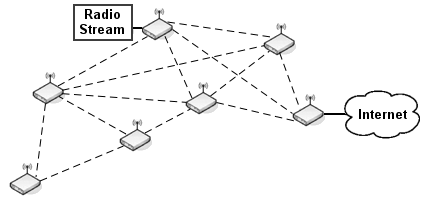
\includegraphics[width=\textwidth]{images/mesh_uebersicht.png}   
		\end{column}
	\end{columns} 
\end{frame}


\begin{frame}
\frametitle{Wohin geht welcher Traffic?}
	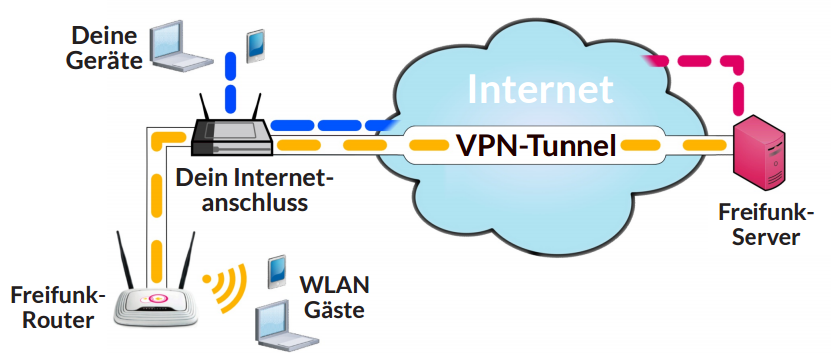
\includegraphics[scale=0.4]{images/personal_setup.png}
\end{frame}

\subsection{Juristisches}

\begin{frame}
\frametitle{Störerhaftung}
	\begin{itemize}
		\item Keine Probleme durch Störerhaftung, da VPN Tunnel zu unserem Verein, dem Community Provider F3Netze e.V.
		\item Negativen Feststellungsklagen gegen die Störerhaftung \\$\rightarrow$ Erste Erfolge beim Arbeitsgericht Charlottenburg
		\item Gesetzesentwurf der Regierung zur Störerhaftung geplant \\$\rightarrow$ Bekannter Entwurf unzureichend \href{http://freifunkstattangst.de/2015/03/05/tmg-gesetzesentwurf-wuerde-zu-mehr-rechtsunsicherheit-und-negativen-effekt-auf-die-verbreitung-von-funknetzwerken-fuehren/}{(Stellungnahme)}
	\end{itemize}
\end{frame}

\section{Technik}


\subsection{Test1}
\begin{frame}



\begin{block}{Hallo}

i bims
\end{block}

\begin{itemize}
\item Test
\item Test2
\end{itemize}
\end{frame}


\subsection{Test2}
\begin{frame}

\begin{itemize}
\item Test
\item Test2
\end{itemize}
\end{frame}
\section{Die Community}
\subsection{Status des Projekts}

\begin{frame}
\frametitle{Status Deutschland}
	\begin{columns}[c]   
		\begin{column}[T]{0.6\textwidth}     
			\begin{itemize}
				\item ca. 280 Communities \footnotemark[1]
				\item ca. 30.000 Access Points \footnotemark[1]
				\item Offizl. Staatliche Unterstützung:
				\begin{itemize}
					\item Pfalz, Sachsen-Anhalt, Nordrhein-Westfalen 
				\end{itemize}
				\item Offizl. Städtische Unterstützung:
				\begin{itemize}
					\item Berlin, Dresden, Magdeburg, Arnsberg, Osnabrück, Bochum, Mainz, München, Erlangen usw...
				\end{itemize}
			\end{itemize}
		\end{column}
		\begin{column}[T]{0.4\textwidth}     
			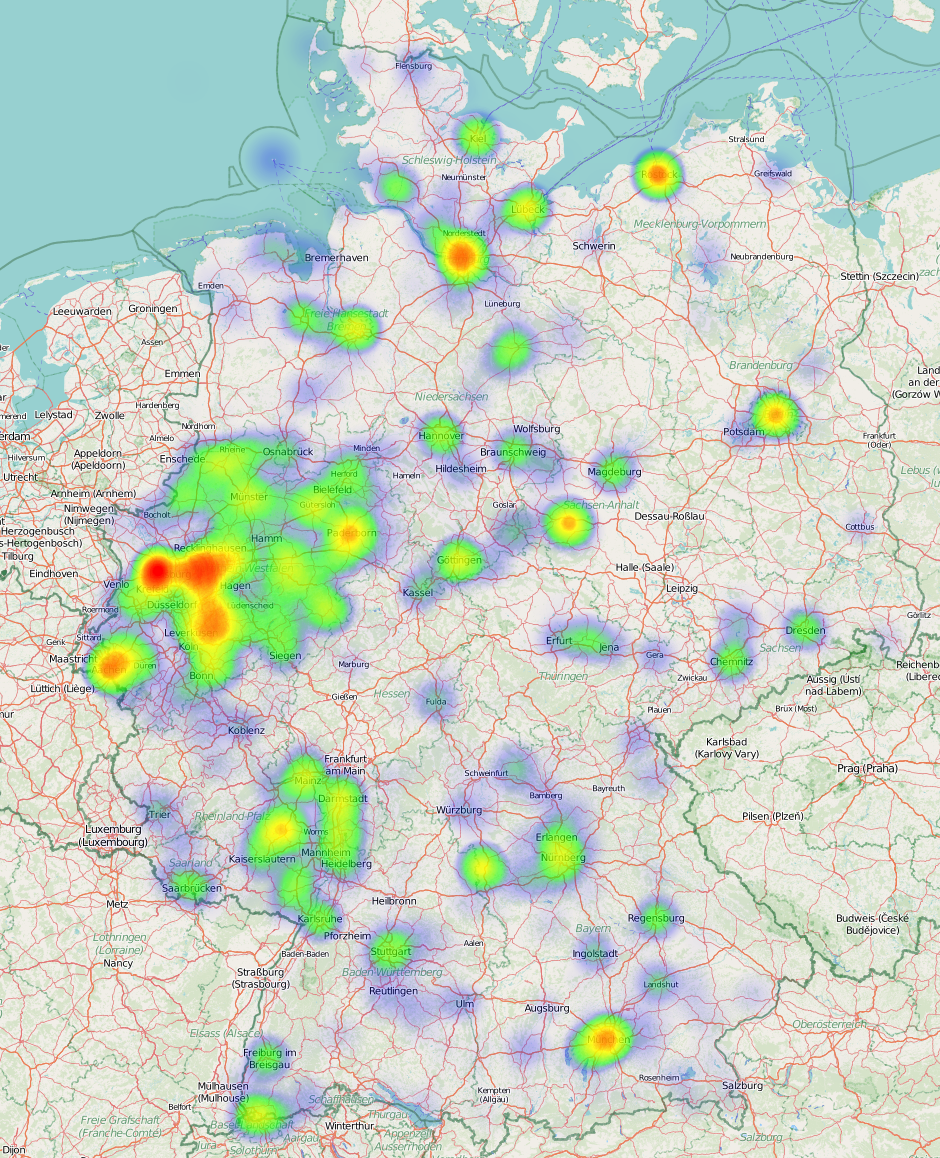
\includegraphics[width=\textwidth]{images/heatmap_germany.png} 
		\end{column}
	\end{columns}		
	\footnotetext[1]{Stand: 12.03.2016}

\end{frame}

\begin{frame}
\frametitle{Status Franken}
	\begin{itemize}
		\item ca. 50-300 aktive Freifunker: per eMail erreichbar und in der Mailingliste/Wiki aktiv
		\item etwa 2000 online Knoten
			\begingroup 
				\tiny{Stand 11.06.2017}
			\endgroup
		\item Ständig 3-4k Clients  
			\begingroup 
				\tiny{Stand 11.06.2017 - \href{https://monitoring.freifunk-franken.de/statistics}{Live Daten (Monitoring)}}
			\endgroup
	\end{itemize}
	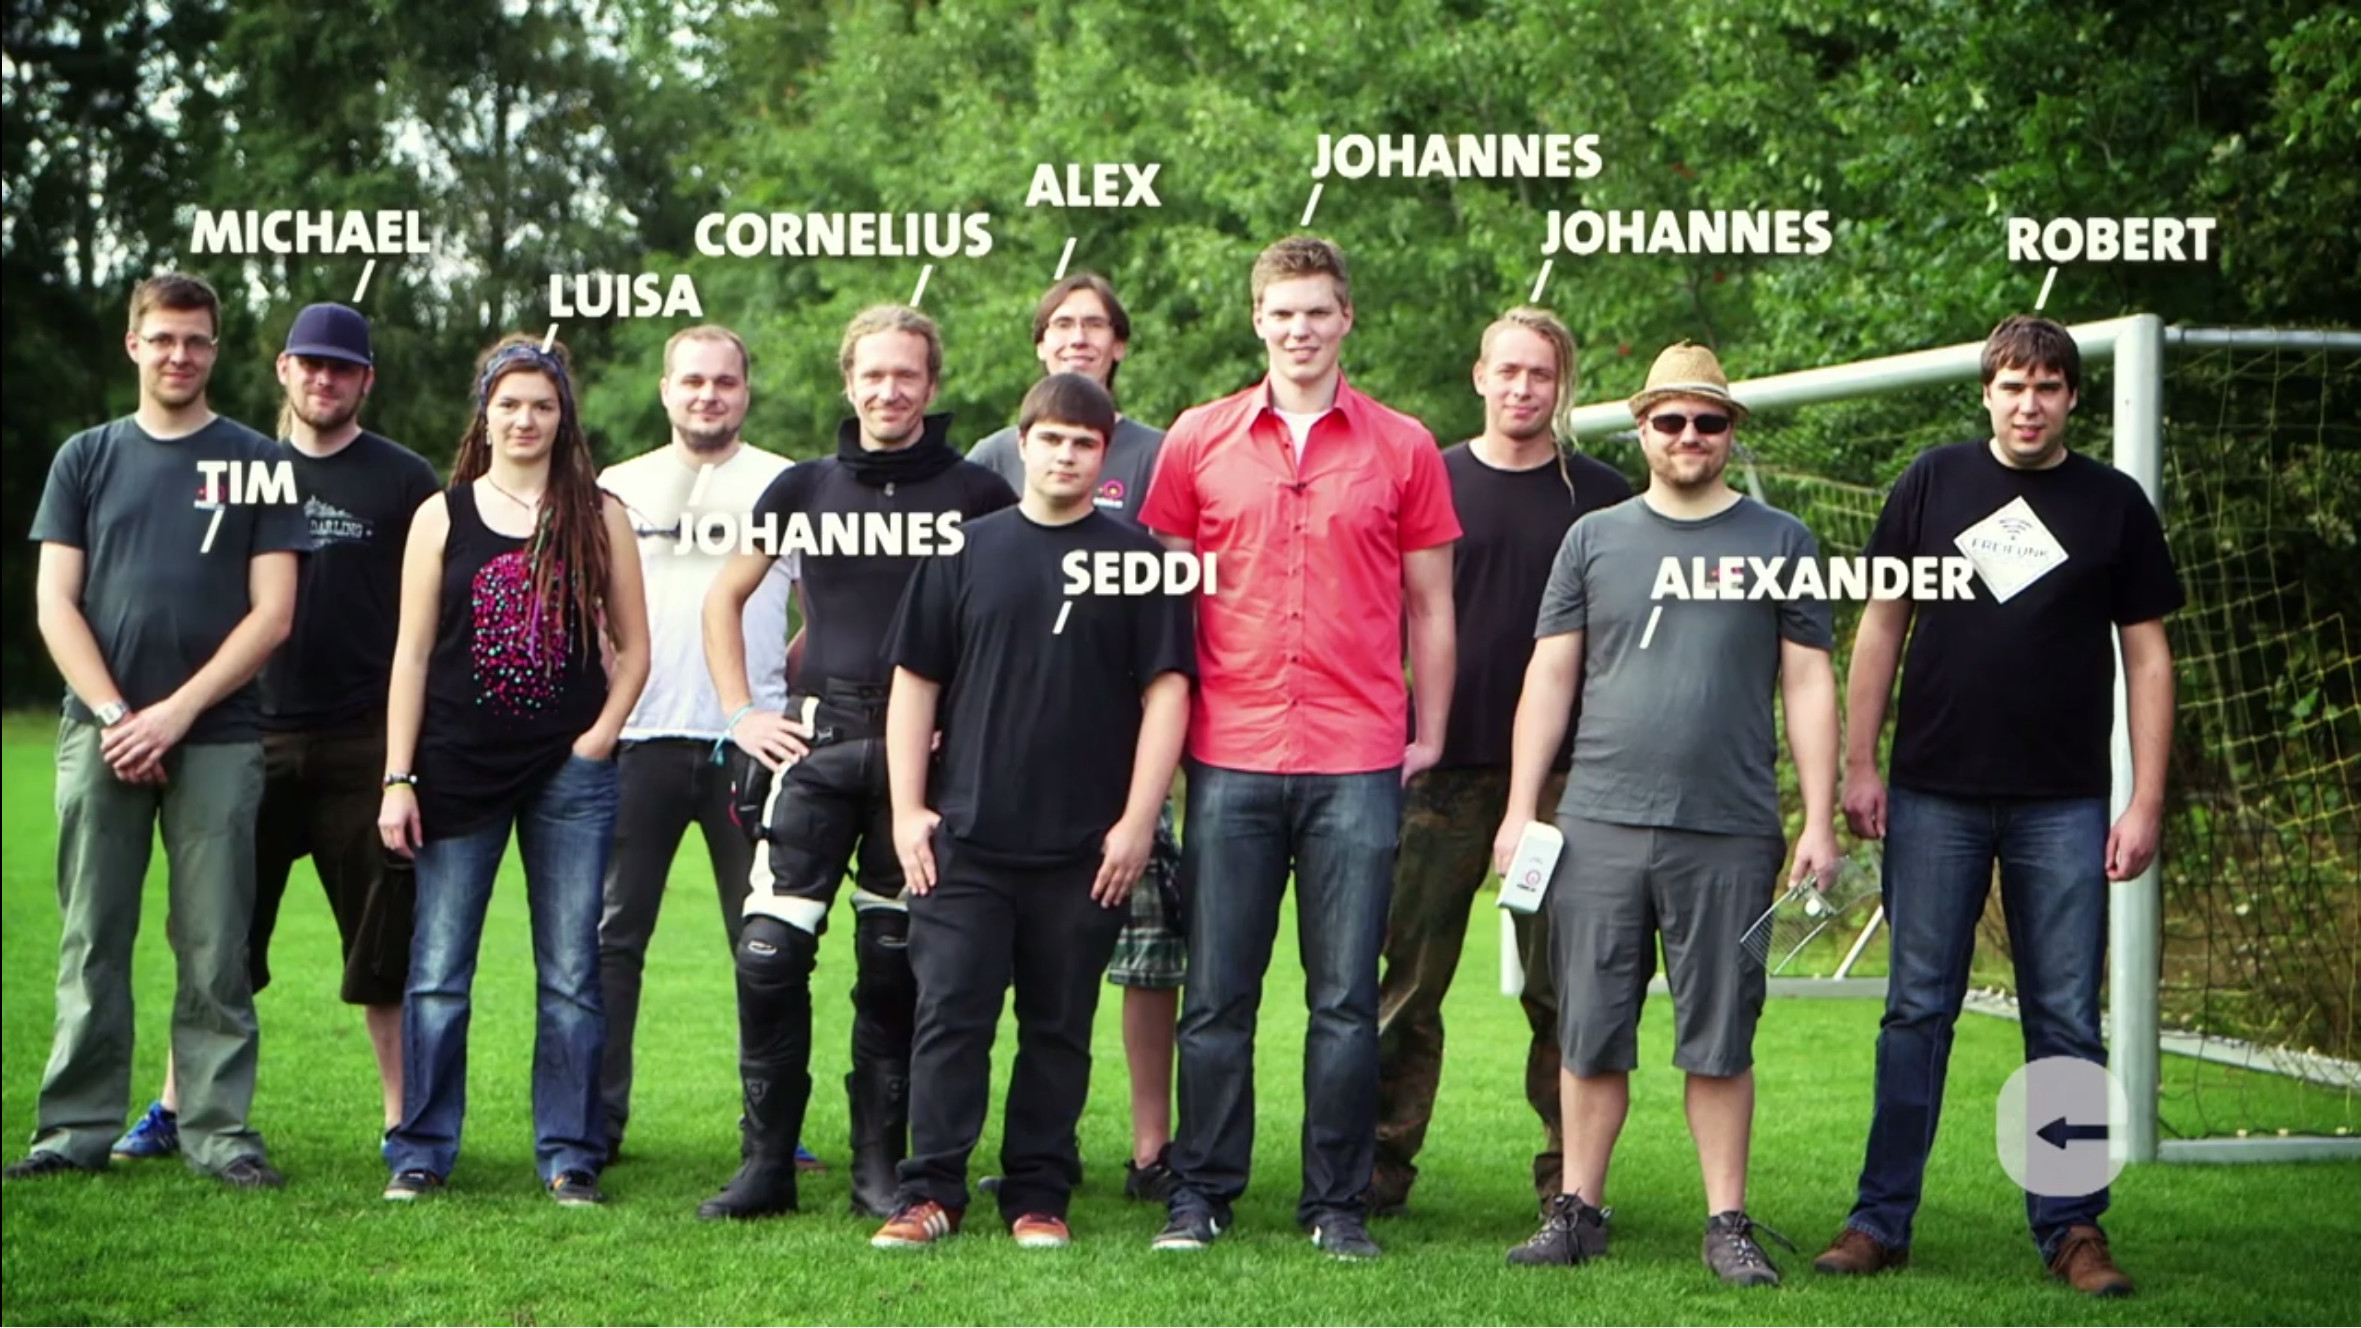
\includegraphics[width=\textwidth]{images/community.jpg}
\end{frame}

\subsection{Mitmachen!}

\begin{frame}
\frametitle{Mitmachen!}
	\begin{itemize}
		\item Anleitung gibt es im eigenen Wiki 
			\\ \href{https://wiki.freifunk-franken.de/w/Mitmachen}{https://wiki.freifunk-franken.de/w/Mitmachen}
		\item Mailingliste 
			\\ \href{https://wiki.freifunk-franken.de/w/Kommunikation}{https://wiki.freifunk-franken.de/w/Kommunikation}
		\item Netzverwaltung mit Karte: 
			\\ \href{https://monitoring.freifunk-franken.de}{https://monitoring.freifunk-franken.de}
	\end{itemize}
	\begin{flushright}
		
\includegraphics[scale=0.7]{images/CC-BY-SA.png}
		\begingroup \tiny{		
			\\CC-BY-SA März 2016 by delphiN, Casandro
			\\CC-BY-SA Mai 2016/Juni 2017 by b3yond
			\\CC-BY-SA Juni 2017 by MikeTsenatek
			\\CC-BY-SA November 2015 by RedDog}
		\endgroup
	\end{flushright}
\end{frame}




\end{document}
